\section{Meios Porosos}

Cada ambiente sedimentar possui diferentes características em relação à forma e ao tipo de sedimento. Tais diferenças, notoriamente, influenciam diretamente no movimento do fluido no interior do meio poroso. Sendo assim, para modelar escoamentos em rochas sedimentares é necessário descrever a geometria e as propriedades físicas das rochas e dos fluidos envolvidos \cite{Ahmed2010}. Por um lado, as propriedades físicas da rocha que compõe o meio poroso refletem a capacidade da mesma de transmitir e acumular fluidos em seus poros. As propriedades físicas (intensivas ou extensivas) do fluido, por outro, permitem descrever mudanças entre estados momentâneos, os quais ocorrem em detrimento de um desequilíbrio termodinâmico\footnote{O equilíbrio termodinâmico é definido quando todas as propriedades de um sistema forem constantes e uniformes. Em outras palavras, quando há: equilíbrio térmico (uniformidade e invariância na temperatura), mecânico (uniformidade e invariância na pressão) e químico (uniformidade e invariância nas concentrações das espécies químicas). Naturalmente, o desequilíbrio termodinâmico ocorre quando ao menos um dos itens referidos acima não é satisfeito \cite{Borgnakke2018}.} do sistema em análise. Em geral, propriedades físicas dos fluidos como massa específica, viscosidade e compressibilidade variam com a pressão do reservatório, o que influencia diretamente as características do escoamento no interior do meio poroso.  

\subsection{Definição}

O material que compõe o meio poroso pode variar desde areia muito solta e não consolidada a rochas sedimentares muito dura e densas, como o arenito, o calcário e a dolomita \cite{Ahmed2010}. A composição sedimentar do meio poroso, nesse sentido, influencia de forma significativa as propriedades físicas do mesmo, \textit{e.g.} porosidade, permeabilidade e saturação. Assim, o conhecimento das propriedades físicas do meio poroso e a interação deste com os fluidos e fases em seu interior são fundamentais para avaliar a viabilidade de um reservatório de petróleo.   

\subsection{Propriedades físicas dos meios porosos}

A caracterização de um meio poroso, tal como referido anteriormente, sucede-se das propriedades físicas do mesmo. Nesse aspecto, define-se, a seguir, os conceitos de porosidade, permeabilidade e saturação. 

\subsubsection{Porosidade}

A porosidade de um meio poroso consiste na capacidade de armazenar fluidos. Quantitativamente, a porosidade é definida pela fração do volume de poros ou a fração de vazio da formação \cite{Ahmed2010,Sousa2023}. Assim sendo, a porosidade, $\phi$, é expressa matematicamente como:

\begin{equation}
	\phi = \frac{V_{p}}{V_{t}},
\end{equation}

onde $V_{p}$ denomina o volume de vazios da rocha e $V_{t}$ o volume total da mesma \cite{Rosa2006}. Desta forma, é imediato observar que a porosidade é uma grandeza adimensional, a qual assume valores entre zero e a unidade. A fração do reservatório ocupada pela rocha é, portanto, $1-\phi$. Note que a definição acima não faz distinção entre os poros que estão interconectados, ou seja, que de fato permitem o escoamento de fluidos e aqueles que estão desconectados. Por esse motivo, a porosidade, tal como definida acima, é designada absoluta. A porosidade efetiva, por sua vez, é definida como a fração do volume de poros interconectados na rocha e o volume total da mesma, \textit{i.e.}:

\begin{equation}
	\phi_{ef} = \frac{V_{p,int}}{V_{t}}.
\end{equation}

Em verdade, em cenários reais, a porosidade é medida em ensaios laboratoriais a partir de pequenas amostrar de rochas. O valor da porosidade do reservatório como um todo é, então, estimado estatisticamente por meio dos resultados de análises conduzidas em uma grande quantidade de amostras \cite{Sousa2023}. Vale destacar, ademais, que um meio poroso pode ser classificado em incompressível ou compressível. O primeiro é caracterizado por uma porosidade estática; o segundo, por uma porosidade dinâmica. Neste último, a porosidade é função da pressão termodinâmica do reservatório e a dependência decorre da compressibilidade do meio poroso, $c_{r}$, a qual relaciona a variação do volume com a pressão $p$ no mesmo:

\begin{equation}
	c_{r} = \frac{1}{\phi}\frac{d \phi}{dp} = \dfrac{d\ln{\phi}}{dp}.
\end{equation}

Sob a hipótese de compressibilidade constante, a equação acima pode ser integrada e culmina na seguinte expressão:

\begin{equation}
	\phi(p) = \phi_{0}e^{c_{r}(p-p_{0})}.
\end{equation}

Naturalmente, fazendo-se uso da expansão em série de Taylor da função exponencial, pode-se aproximar a porosidade como função linear da pressão, ou seja, 

\begin{equation}
	\phi(p) \approx [1+c_{r}(p-p_{0}].
\end{equation}

\subsubsection{Permeabilidade}

A permeabilidade, $\mathbf{K}$, do meio poroso corresponde a capacidade da formação em transmitir fluidos através de seus poros interconectados \cite{Chen2006,Sousa2023}. Esta propriedade é de suma importância para a correta caracterização do reservatório, visto que controla o movimento direcional e a vazão dos fluidos na formação. Este parâmetro foi inicialmente introduzido por Henry Darcy em 1856 em sua então denominada Lei de Darcy \cite{Ahmed2010}. 

Na presença de um único componente e uma única fase, a permeabilidade é designada absoluta. Sua unidade no SI é dada em $[\text{m}^{2}]$, muito embora seja comumente expressa em unidade de Darcy [D]\footnote{Nota: $1\text{D} \approx 0,987 \times 10^{-12}\text{m}^{2}$.} ou mili-Darcy [mD]. Rochas com poros grande e bem conectados resultam em uma permeabilidade alta, como ocorre, em geral, nos arenitos. Noutra vertente, rochas com poros menores e pouco conectados possuem baixa permeabilidade e são frequentemente denominados de rochas impermeáveis \cite{Sousa2023}. 

A permeabilidade absoluta, $\mathbf{K}$, é definida através de um tensor de segunda ordem simétrico positivo definido:

\begin{equation}
	\mathbf{K} = \begin{bmatrix}
		k_{xx} & k_{xy} & k_{xz} \\
		k_{yx} & k_{yy} & k_{yz} \\
		k_{zx} & k_{zy} & k_{zz}
	\end{bmatrix}.
\end{equation}

Neste caso, os termos da diagonal principal delimitam a relação entre a vazão em uma direção axial e o gradiente de pressão na mesma direção. Os elementos fora da diagonal, portanto, estabelecem a relação entre a vazão e gradiente de pressão em direções perpendiculares. Neste cenário, o tensor é dito anisotrópico. Em contrapartida, quando $K_{xx} = K_{yy} = K_{zz}$, o tensor é dito isotrópico e a permeabilidade passa a ser expressa por um escalar. Notoriamente, quando a permeabilidade do meio poroso é dita uniforme, a formação é dita homogênea; caso contrário, é dita heterogênea. Este último caso, outrossim, é mais frequente e deve-se, sobretudo, as diferentes partículas existentes no meio poroso, ao nível de cimentação e a transição entre diferentes formações rochosas.

\subsubsection{Saturação}


\subsection{Propriedades físicas dos fluidos}

\subsection{Volumes elementares representativos}

\subsection{Leis constitutivas para escoamento em meios porosos}

\subsubsection{Lineares}

\paragraph{Modelo de Darcy}

A lei constitutiva de Darcy, como fora referida outrora, advém do estudo realizado pelo físico francês Hanry Darcy, em 1856. Em seu trabalho, Hanry Darcy investigou os sistemas hidrológicos de suprimento de água na cidade de Dijon, na França. Para tanto, performou uma análise sobre o fluxo de água unidimensional e em regime permanente em colunas de areia uniforme \cite{Darcy1856}. A figura \ref{fig:Darcy_experiment} ilustra esquematicamente o aparato experimental empregado. 

\begin{figure}[!ht]
	\centering
	\caption{Experimento de Darcy.}    
	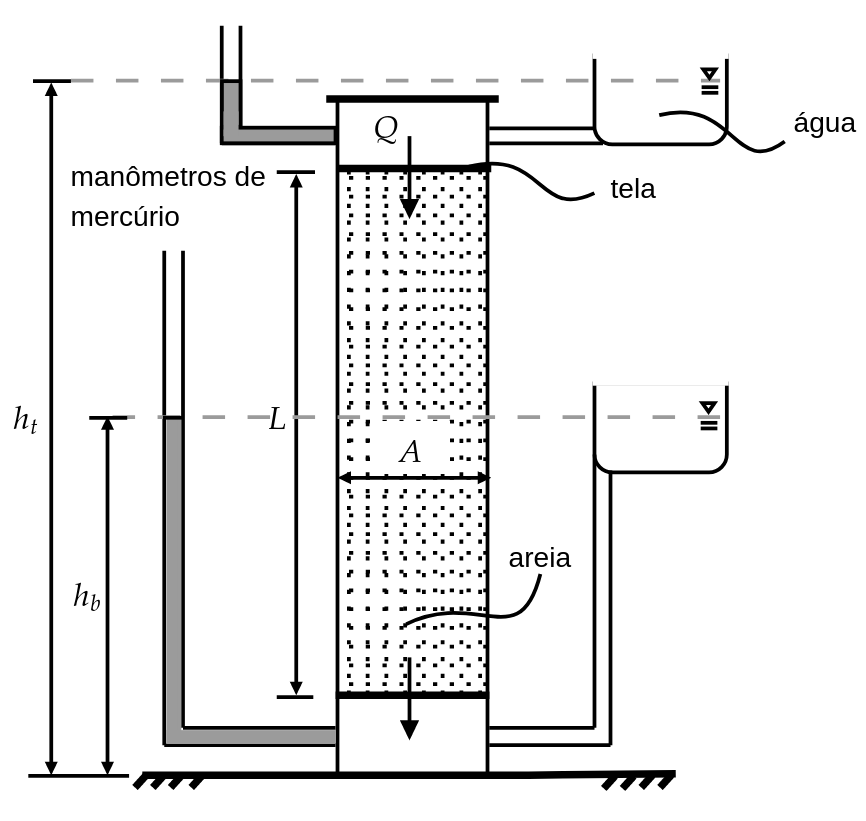
\includegraphics[width=0.5\textwidth]{Figuras/Gerais/Darcy_experiment.png}
	\caption*{Fonte: autor.}
	\label{fig:Darcy_experiment}
\end{figure}

A partir do experimento, Darcy pôde concluir que o fluxo volumétrico, $Q$ (volume por unidade de tempo), era diretamente proporcional à área de seção transversal, $A$, à diferença $h_{t}-h_{b}$ e inversamente proporcional à altura da coluna de areia, $L$. Matematicamente, tem-se que:

\begin{equation}
	\frac{Q}{A} = - k \frac{h_{b}-h_{t}}{L}\mathbf{\hat{e}}_{z},
\end{equation}

onde $\mathbf{\hat{e}}_{z}$ corresponde ao vetor normal unitário na direção do escoamento e $k$ é a condutividade hidráulica do meio, admitido como isotrópico e homogêneo. Nesse sentido, para o caso particular, a condutividade hidráulica\footnote{Note que a condutividade hidráulica, ao contrário da permeabilidade absoluta, depende tanto das propriedades do meio poroso quanto das do fluido que escoa através do mesmo.} é definida como $k = \frac{\rho g K}{\mu}$, onde $\mu$ denomina a viscosidade dinâmica do fluido. Alguns autores, \textit{e.g.} \cite{Sousa2023}, denominam a razão $\frac{Q}{A}$ como sendo o fluxo de Darcy, $\mathbf{q}$; outros -- \textit{e.g.} \cite{Jambhekar2011} --, contudo, optam por denominar velocidade de Darcy, $\mathbf{u}$; neste último caso, no entanto, deve-se salientar que como apenas uma fração da área da seção transversal é considerada para o fluxo, em detrimento da presença dos grãos de areia, $\mathbf{u}$ corresponde a uma velocidade macroscópica média dos fluxos microscópicos que ocorrem no interior de REVs \cite{Sousa2023,Freeze1979}.     

A extensão da equação acima para o caso mais geral, \textit{i.e.}, tridimensional, anisotrópico e heterogêneo ocorre de maneira imediata, como se segue:

\begin{equation}
	\mathbf{u} = - \frac{\rho g}{\mu} \mathbf{K} \cdot \nabla h, 
\end{equation}

onde $\mathbf{K}$ é o tensor permeabilidade absoluta do meio e $h$ corresponde à queda piezométrica, ou seja,

\begin{equation}
	h = \frac{p}{\rho g} + z,
\end{equation}

em que $p$ é a pressão termodinâmica, $\rho$ é a massa específica do fluido e $g$ é a aceleração gravitacional local. Levando-se a equação (3.9) na equação (3.8), resulta que:

\begin{equation}
	\mathbf{u} = -\frac{\mathbf{K}}{\mu} \cdot (\nabla p + \rho g \nabla z)
\end{equation}

Em coordenadas cartesianas e definindo $\mathbf{\hat{e}}_{z}$ vertical para cima, a equação (3.10) pode ser reescrita na forma:

\begin{equation}
	\mathbf{u} = - \frac{\mathbf{K}}{\mu} \cdot (\nabla p - \rho \mathbf{g}),
\end{equation}

em que $\mathbf{g} = -g\mathbf{\hat{e}}_{z}$. 

A equação de Darcy possui aplicações nas mais diversas áreas da engenharia e da física, incluindo, por exemplo: escoamento em meios porosos \cite{Bear2013}, escoamento em aquíferos e aquitardos ou águas subterrâneas \cite{Atangana2018}. No entanto, a equação de Darcy é válida segundo um conjunto de hipóteses: escoamento em regime laminar, estacionário, isotérmico e incompressível; meio poroso saturado e, por fim, ausência de variações de energia cinética macroscópica \cite{Freeze1979}.

Dentre as hipóteses referidas, detalha-se aquela associada ao regime laminar do escoamento. Nesse sentido, o escoamento deve ser caracterizado pelo domínio das forças viscosas sobre as inerciais. A razão entre forças inerciais e forças viscosas é definida através do número de Reynolds (Re) \cite{Pontes2016}. O número de Re é o adimensional responsável por caracterizar três diferentes padrões de escoamento: laminar, transicional e turbulento e é definido, para cenário de meios porosos como:

\begin{equation}
	\text{Re} = \frac{\text{Forças inerciais}}{\text{Forças viscosas}} = \frac{\rho ||\mathbf{u}|| L}{\mu},
\end{equation}

onde $\rho$ e $\mu$ delimitam a massa específica e a viscosidade dinâmica do fluido, respectivamente, $||\mathbf{u}||$ é o módulo da velocidade do escoamento e $L$ é um comprimento característico, em geral, associado aos REVs. Nesse viés, a equação de Darcy é aplicável, conforme apresentado em \cite{Bear2013}, para $\text{Re} \leq 10 $

\begin{figure}[!ht]
	\centering
	\caption{...}
	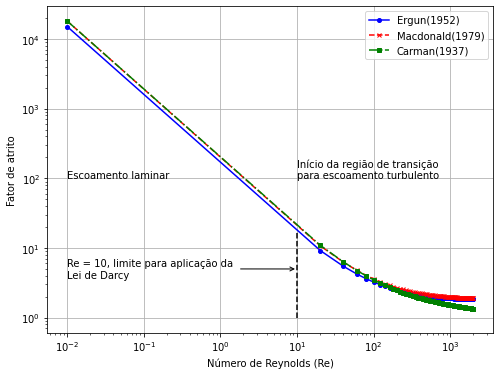
\includegraphics[width=0.75\linewidth]{Figuras/Gerais/Darcy_law_graph.png}
	\caption*{Fonte: autor.}
	\label{fig:Darcy_law_graph}
\end{figure}


\subsubsection{Não lineares}

\paragraph{Modelo de Forchheimer}

\textcolor{red}{Após mencionar o número de Re limite, para o qual a Lei de Darcy é aplicável, introduzir-se-á o modelo de Forcheimer}




